\documentclass[11pt]{article}

\usepackage{times,epsf,epsfig,textcomp,amsmath,amssymb,subfigure,wrapfig,cite,moreverb}
\usepackage{comment}
\usepackage{array}
\usepackage{colortbl}
\usepackage{url}
\usepackage{color,soul}
\usepackage[dvipsnames]{xcolor}
\usepackage[normalem]{ulem}
\usepackage{graphics}
\usepackage{listings}
\usepackage{paralist}
\usepackage{todonotes}
\usepackage{xspace}
%\usepackage[bookmarks, breaklinks=true, colorlinks=true, plainpages = false,
%  citecolor = blue, urlcolor = blue, filecolor = blue,]{hyperref}

\usepackage[labelfont=bf,font=small]{caption}
\usepackage{multirow}

\definecolor{tableYellow}{rgb}{.996, 1, .8549}
\definecolor{tableBlue}{rgb}{0.8823, .9098, 1}
\definecolor{tableRed}{rgb}{1, .9255, .9019}
\definecolor{tableGreen}{rgb}{.9176, 1, .9216}
\definecolor{tableGray}{rgb}{.902, .902, .902}
\definecolor{dragos}{rgb}{1,0.5,0}
\setcounter{tocdepth}{2}
\def\tablestrut{\vrule height1.25em depth0pt width0pt}
\def\topfraction{.9}
\def\bottomfraction{.9}
\def\textfraction{.1}

\textheight 8.7in \textwidth 6.5in \oddsidemargin +0in \evensidemargin
0in \topmargin -.3in \advance \topmargin-\baselineskip \headsep .5in
\marginparwidth .7in \marginparsep .15in

\floatsep 8pt plus 2pt minus 2pt \textfloatsep 8pt plus 2pt minus
2pt

\makeatletter
\renewcommand\section{\@startsection {section}{1}{\z@}%
   {-3ex \@plus -1ex \@minus -.2ex}%
   {1.7ex \@plus.2ex}%
   {\normalfont\large\bfseries}}
\renewcommand\subsection{\@startsection{subsection}{2}{\z@}%
   {-2.5ex\@plus -1ex \@minus -.2ex}%
   {1ex \@plus .2ex}%
   {\normalfont\normalsize\bfseries}}
\renewcommand\subsubsection{\@startsection{subsubsection}{2}{\z@}%
   {-1ex\@plus -1ex \@minus -.2ex}%
   {0.3ex \@plus .2ex}%
   {\normalfont\normalsize\bfseries}}

\newcommand\minisection{\@startsection{subsubsection}{4}{\z@}%
   {1ex\@plus 0ex \@minus 0ex}%
   {-1.5ex \@plus .2ex}%
   {\normalfont\normalsize\bfseries}}

\setcounter{secnumdepth}{2} \makeatother



%------------Formatting----------
\newcommand{\Paragraph}[1]{\vskip 6pt\noindent\textbf{#1. }}
\newcommand\paratitle[1]{\textit{\textbf{#1}}}
\newcommand\itno[1]{({\em #1})}
\newcommand\itemno[1]{({\em #1})}

\newcommand\copyfromuser{\url{copy_from_user}}
\newcommand\copytouser{\url{copy_to_user}}
\newcommand\mappage{\url{map_page}}
\newcommand\unmappage{\url{unmap_page}}

%%%%%%%%%%%%%%% smitemize %%%%%%%%%%%%%%%%%%%%

\newenvironment{smitemize}%
  {\begin{list}{$\bullet$}%
     {\setlength{\parsep}{0pt}%
      \setlength{\topsep}{0pt}%
      \setlength{\itemsep}{2pt}}}%
  {\end{list}}

%%%%%%%%%%%%%%% custom spacing %%%%%%%%%%%%%%%%%%%%

\newcommand{\customvspace}{\vspace{0in}}
\newcommand{\customvspacetwo}{\vspace{0.01in}}
\newcommand{\intercolumnhspace}{\hspace{0.64cm}} % the intercolumn spacing


% !TEX root = main.tex
%----------- Comments-----------------
\newcommand{\hlc}[2][yellow]{ {\sethlcolor{#1} \hl{#2}} }
\newcommand\note[1]{\hlc[SkyBlue]{-- #1 --}} % highlighted notes of other colors.
						 % For colors info from xcolor package, check out:
						 % http://en.wikibooks.org/wiki/LaTeX/Colors
\newcommand\lin[1]{\hlc[yellow]{Lin:-- #1 --}}
\newcommand\yy[1]{\hlc[LimeGreen]{Yanyong: #1}}
%%%%%%%%%%%%%%% footnote %%%%%%%%%%%%%%%%%%%%

%\renewcommand\footnote[1]{} % remove footnotes

%%%%%%%%%%%%%%% candidate %%%%%%%%%%%%%%%%%%%%

%\newcommand\candidate[1]{#1} %put text back normally
\newcommand\candidate[1]{} %remove text
%\newcommand\candidate[1]{\hlc[Blue]{----} #1 \hlc[Blue]{----}} % highlight text

\newcommand\candidatetwo[1]{} %remove text




% -------------------Proposal specific TERMS -------------------

\newcommand{\projecttitle}{CPS: Synergy: Collaborative Research: Town Tomography with Many-Antenna Base Stations}
\newcommand{\authors}{Yanyong Zhang, Rutgers University, and Lin Zhong, Rice University}






\begin{document}

\title{\bf \large \projecttitle}

\author{\authors}

\maketitle

\pagenumbering{arabic}
\def\thepage{C-\arabic{page}}

\tableofcontents

\pagebreak \clearpage \pagenumbering{arabic}
\def\thepage{\arabic{page}}
\thispagestyle{empty}

% !TEX root = main.tex

\begin{center}

{\bf \projecttitle}
\vspace{+2ex}
\\ \authors\\
\vspace{+1.5ex}
{{\bf Project Summary}} \\
\end{center}



\subsubsection*{Intellectual Merit}

\subsubsection*{Broader Impacts} 


\vspace{+3mm}
\noindent {\bf Key Words: }










\pagebreak

\pagebreak \clearpage \pagenumbering{arabic}
\def\thepage{\arabic{page}}


\begin{center}
{{\bf \projecttitle}}\\
\vspace{+2mm}
{\large {\bf Project Description}} \\
\end{center}

\graphicspath{{figs/}}

% !TEX root = main.tex
\vspace{-10mm}
\section{Introduction\label{sec:intro}}
\
During natural or human-made disasters, the local infrastructure often becomes unavailable, and it is of paramount importance to develop efficient disaster management systems that can function without any infrastructure support. Central to such a system is the ability to rapidly detect whether there are live humans buried under piles of bricks and triage them. Further, these operations must be carried out in a efficient and cost-effective manner. 




\vspace{4pt}\noindent\textbf{Shortcomings with Existing Solutions:} Existing solutions are insufficient for the following reasons.

\vspace{4pt}\noindent\textbf{Tomography-Based Diaster Management with Many-Antenna Receivers:} In this proposal, we propose to design and develop a diaster management cyber-physical system (CPS) using tomography that is supported by many-antenna receivers.

\vspace{4pt}\noindent\textbf{Intellectual Merit:} In order to support a vision of conducting deep tomography-based disaster management using many-antenna receivers, the proposed effort presents a collaborative effort between a team at the Wireless Information Network Laboratory (WINLAB) at Rutgers University, and a team at Rice University to engage in a systems design and integration effort. The Rutgers team will lead the effort in protocol design and initial evaluation, while the Rice team will lead the effort in prototyping and testbed evaluation. We refer to the proposed tomography-based disaster management cyber-physical system as \emph{TomoMan} in this proposal. TomoMan has the following integral components: ***


As part of the broader impacts of the project, the team will reach out to *** 
\pagebreak


% !TEX root = ./main.tex

\section{Testbed: Many-Antenna Base Stations and Mobile Terminals}\label{sec:testbed}

Much the proposed research activities will leverage ArgosNet, a reconfigurable network research testbed with many-antenna MU-MIMO base stations recently funded by an NSF CRI grant.  
ArgosNet includes a configurable number of many-antenna base stations, ArgosBS, battery-powered mobile terminals based on ArgosMobile, and a server cluster connected to the base stations with high-throughout, precisely synchronized backhaul.  Currently ArgosNet supports real-time communication 2.4/5 GHz. Base stations will be precisely synchronized via the backhaul and cooperate to fully support network functions such as handoff and localization. 


\subsection{Argos: Reconfigurable and Scalable Base Station Architecture}\label{sec:argosv2}

\begin{figure*}[t]
%\vspace{-12mm}
\centering
\begin{minipage}[c]{0.62\textwidth}
\centering
 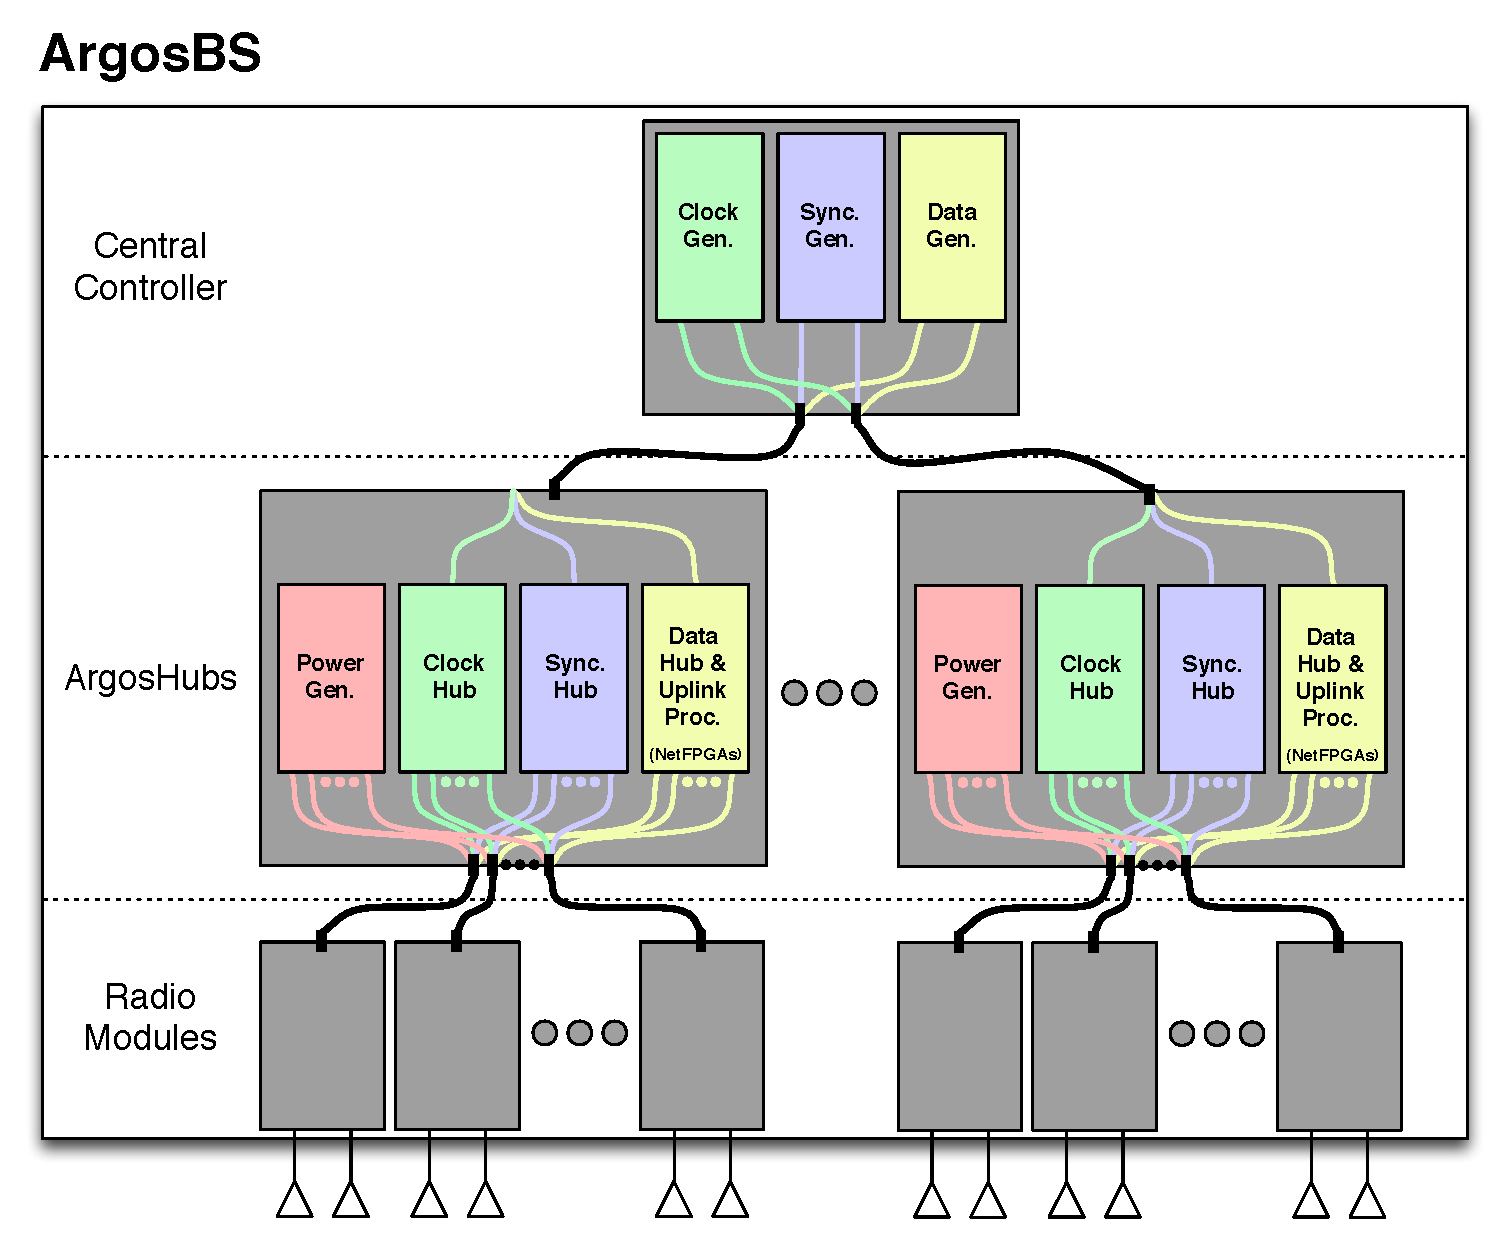
\includegraphics[width=\textwidth]{argosbs}
\end{minipage}
\hspace{2mm}
  \begin{minipage}[c]{0.34\textwidth}
  \centering
 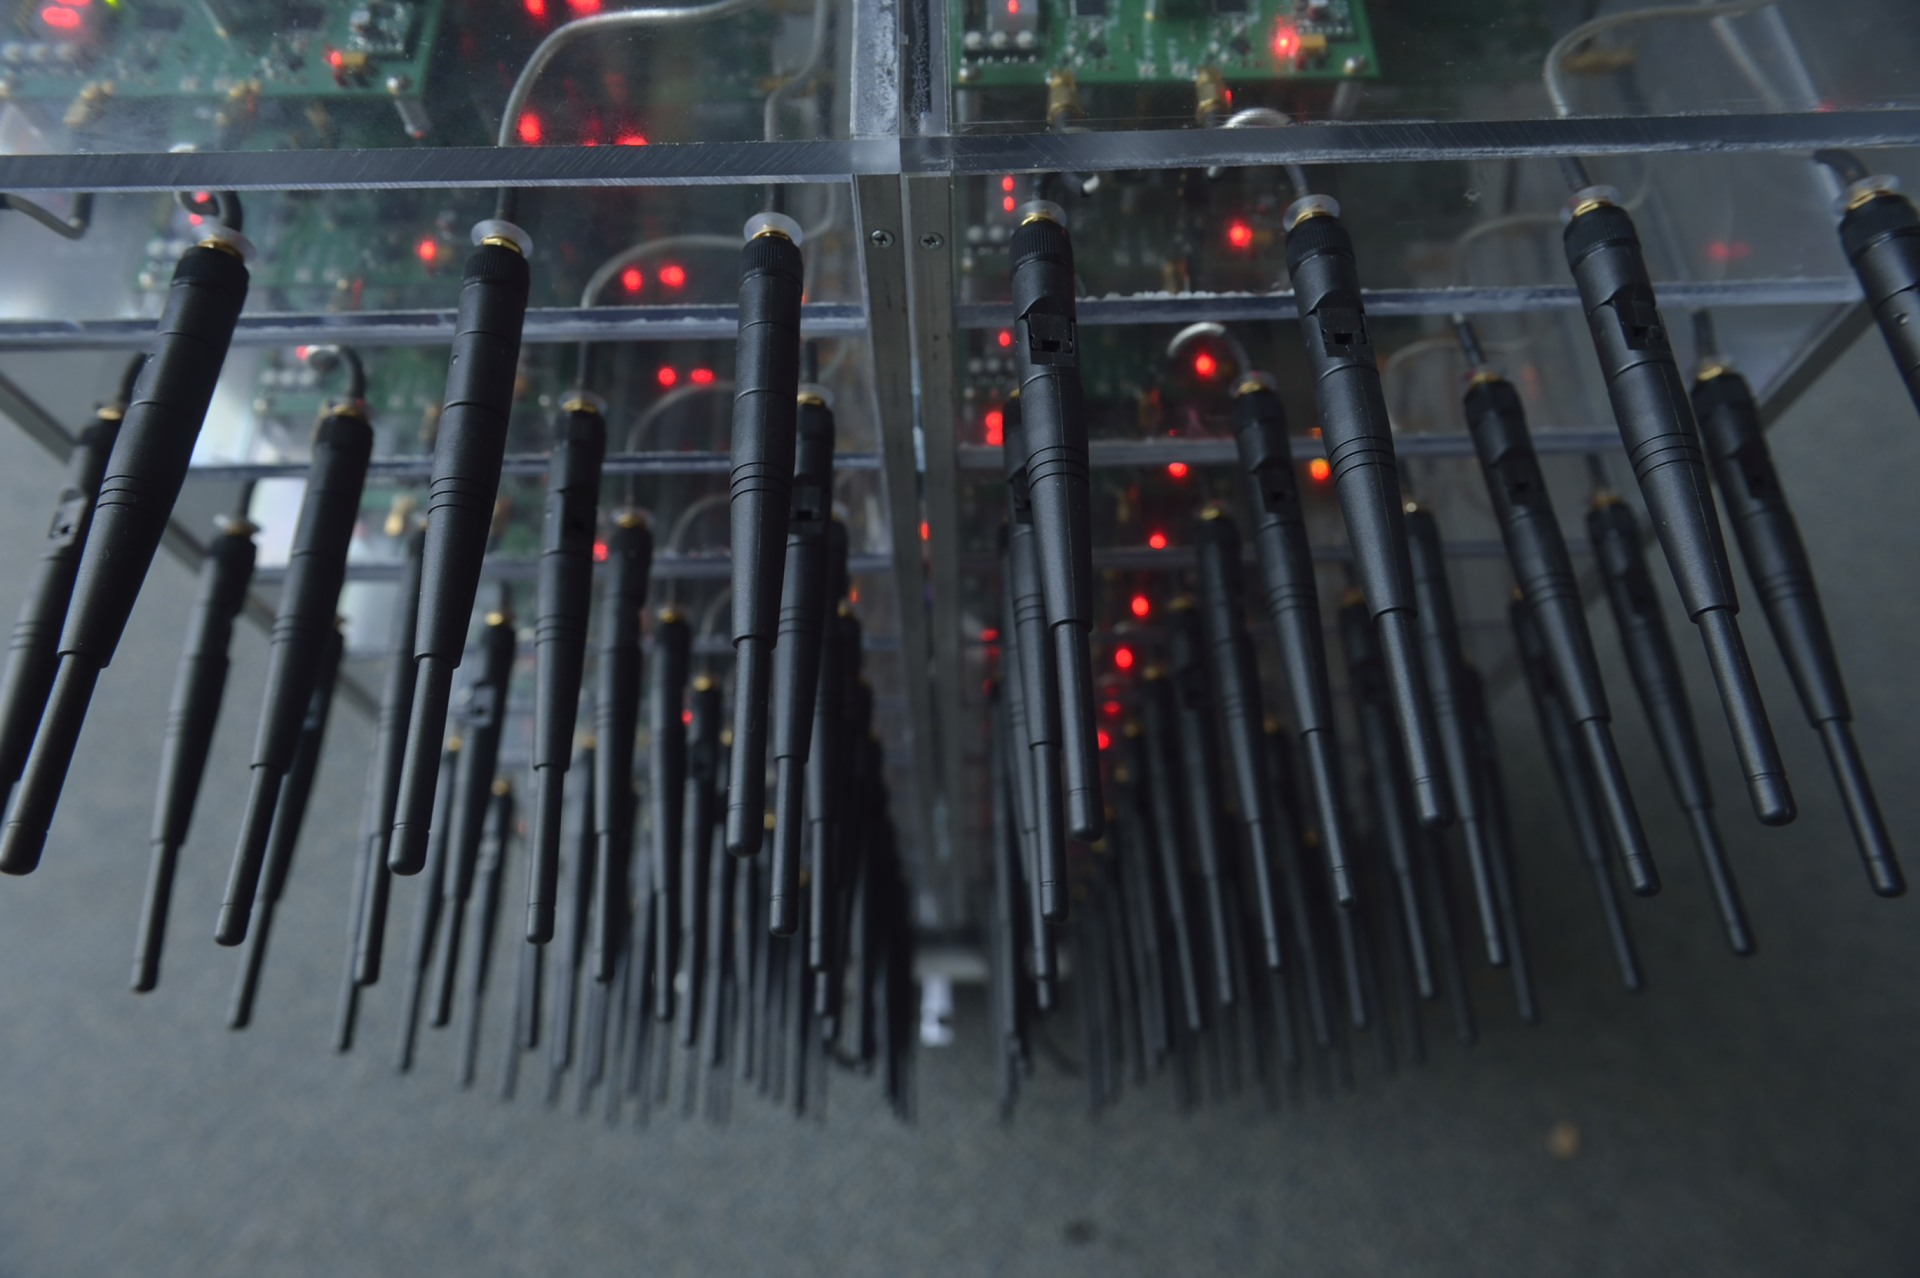
\includegraphics[width=\textwidth]{ArgosV2-Front-full}
 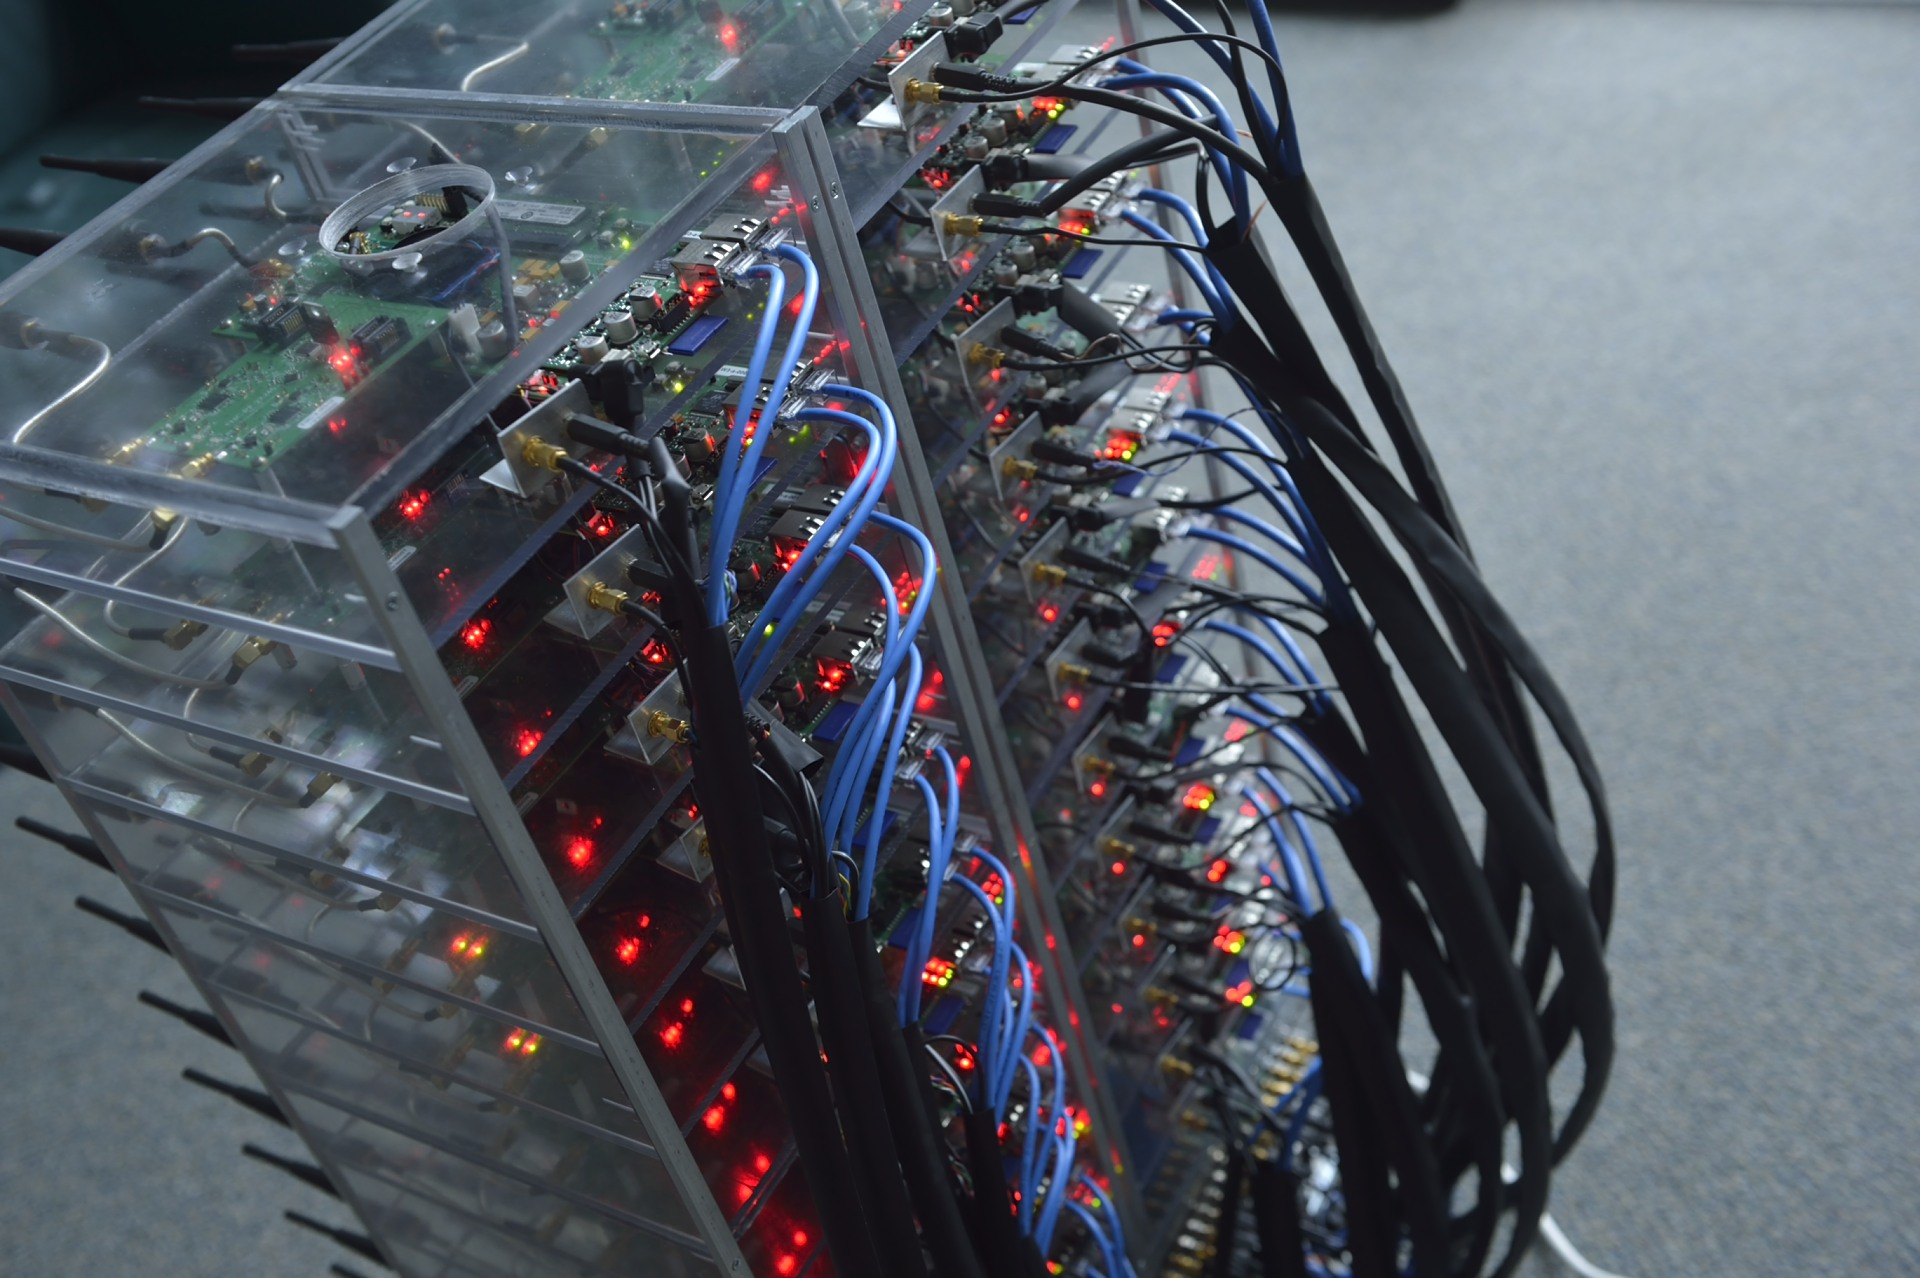
\includegraphics[width=\textwidth]{ArgosV2-Back-full}
 \end{minipage}
		\vspace{-2mm}
\caption{(left): \emph{The architecture of ArgosBS consists of a central controller, one or more ArgosHubs, and up to 100s of radio modules. 
			All links between blocks include a 10 GbE data link, a coaxial clock cable, and a twisted pair for timing synchronization. 
			ArgosHubs additionally supply power to their modules.} (right): \emph{Front and back views of ArgosV2 which features a refined modular mechanical design compared to ArgosV1 reported in~\cite{shepard2012mobicom}.} }
		\vspace{-2mm}
\label{fig:ArgosV2}
\end{figure*}

PI Zhong's group pioneered the design and prototyping of many-antenna base stations, producing two generations of the Argos base station architecture.
The first generation, presented in~\cite{shepard2012mobicom}, employed WARPv1 and supported 64 antennas serving 15 clients via MU-MIMO.  
It provided the first publicly reported experimental results of massive MIMO~\cite{shepard2012mobicom}.
 
The Argos architecture, depicted in Figure~\ref{fig:ArgosV2} (left),  is critical for realizing practical real-world massive-MIMO systems. 
It leverages a fat tree structure to optimize scalability, flexibility, and reliability, allowing massive-MIMO systems to scale to 1000s of antennas in the real world by taking in to account practical constraints. 
At the center of the architecture is the \emph{Central Controller} which is responsible for all layer 2 (MAC), as well as higher-level layer 1 operations, including scheduling, coding, modulation, and portions of MU-MIMO processing.
The central controller is connected to one or more \emph{ArgosHubs}, which distribute user data, maintain synchronization, and perform portions of the MU-MIMO processing such as recombining uplink data streams.
ArgosHubs can be connected to more hubs in a tree topology, for extreme scalability, or directly to the final component, the \emph{Radio Module}.
Radio Modules contain one or more radio interfaces, and perform all required low-level layer 1 computation, such as FFTs and MU-MIMO processing, e.g., precoding.
For additional scalability, Radio Modules can be further connected in series.

The second generation prototype, ArgosV2, recently demonstrated at MobiCom 2013~\cite{ArgosV2} and shown in Figure~\ref{fig:ArgosV2} (right), will serve as base station in ArgosNet.
ArgosV2 fully realizes the hierarchical Argos architecture, and leverages the new WARPv3 to vastly improve the computational capability and backplane throughput of the Radio Module.
It further features a drastically improved mechanical design which enables flexible and rapid reconfiguration of base station components.
ArgosV2 has the following properties that are ideal for ArgosNet. (\textit{i}) Its architecture is scalable to accommodate a large number of antennas; (\textit{ii}) it has adequate computational power distributed among the three major modules; and
(\textit{iii}) It features a flexible modular design, both computationally and mechanically, which enables base stations to quickly and easily re-configured and deployed. 
This design allows base stations to be split in to smaller base stations, or combined in to larger base stations like LEGO bricks, while maintaining distributed computation, protecting the hardware, managing cabling, and facilitating trouble shooting. (\textit{iv}) ArgosV2 is designed to be portable, which allows it to be relocated for testing both indoors and outdoors, or even off-site.  
These capabilities make the platform ideal for rapid prototyping and reconfiguration to support research in everything from completely distribute antenna system to massive-MIMO cellular deployments.

%We will modify our ArgosV2 rack design~\cite{ArgosV2}, shown in Figure~\ref{fig:ArgosV2} to support the new radio modules which include a Volo WSD.
%To maximize flexibility, the new rack will house 9 radio modules, each with 3 SMA connectors, and 1 F-type connector.

\subsection{ArgosMobile}
We have recently created ArgosMobile, an autonomous mobile terminal based on WARPv3 for ArgosV2 base stations. 
Like ArgosBS, it is also completely programmable at all layers of the network stack. 
Its mobility and programmability enable rapid prototyping and experimentation in real-world channels with true mobility. 
To enable mobile applications we leverage a 12V 10AH lithium-ion battery pack, with over a 3 hour life, and a compact and durable custom enclosure shown in Figure~\ref{fig:argosmobile}.
Since feedback and management are critical for rapid development, deployment, and experimentation we employ a dual-band Linksys WET610n Wireless Bridge to provide out-of-band communication to ArgosMobile.
% to connect the ArgosMobile to Rice's existing Wi-Fi network.
 This subtle feature is essential for a research platform, as it enables realistic, real-time, mobile experimentation without having to develop commercial grade wireless stacks, or manage 10s of bulky laptops to control the ArgosMobiles.
Moreover, by connecting the mobiles to Rice's existing network, we are able to seamlessly gain connectivity to the mobiles anywhere on campus to quickly conduct long-range and outdoor experiments.


\begin{figure*}
\centering
%\vspace{-12mm}
\begin{minipage}[t][6.1cm]{0.49\textwidth}
\centering
 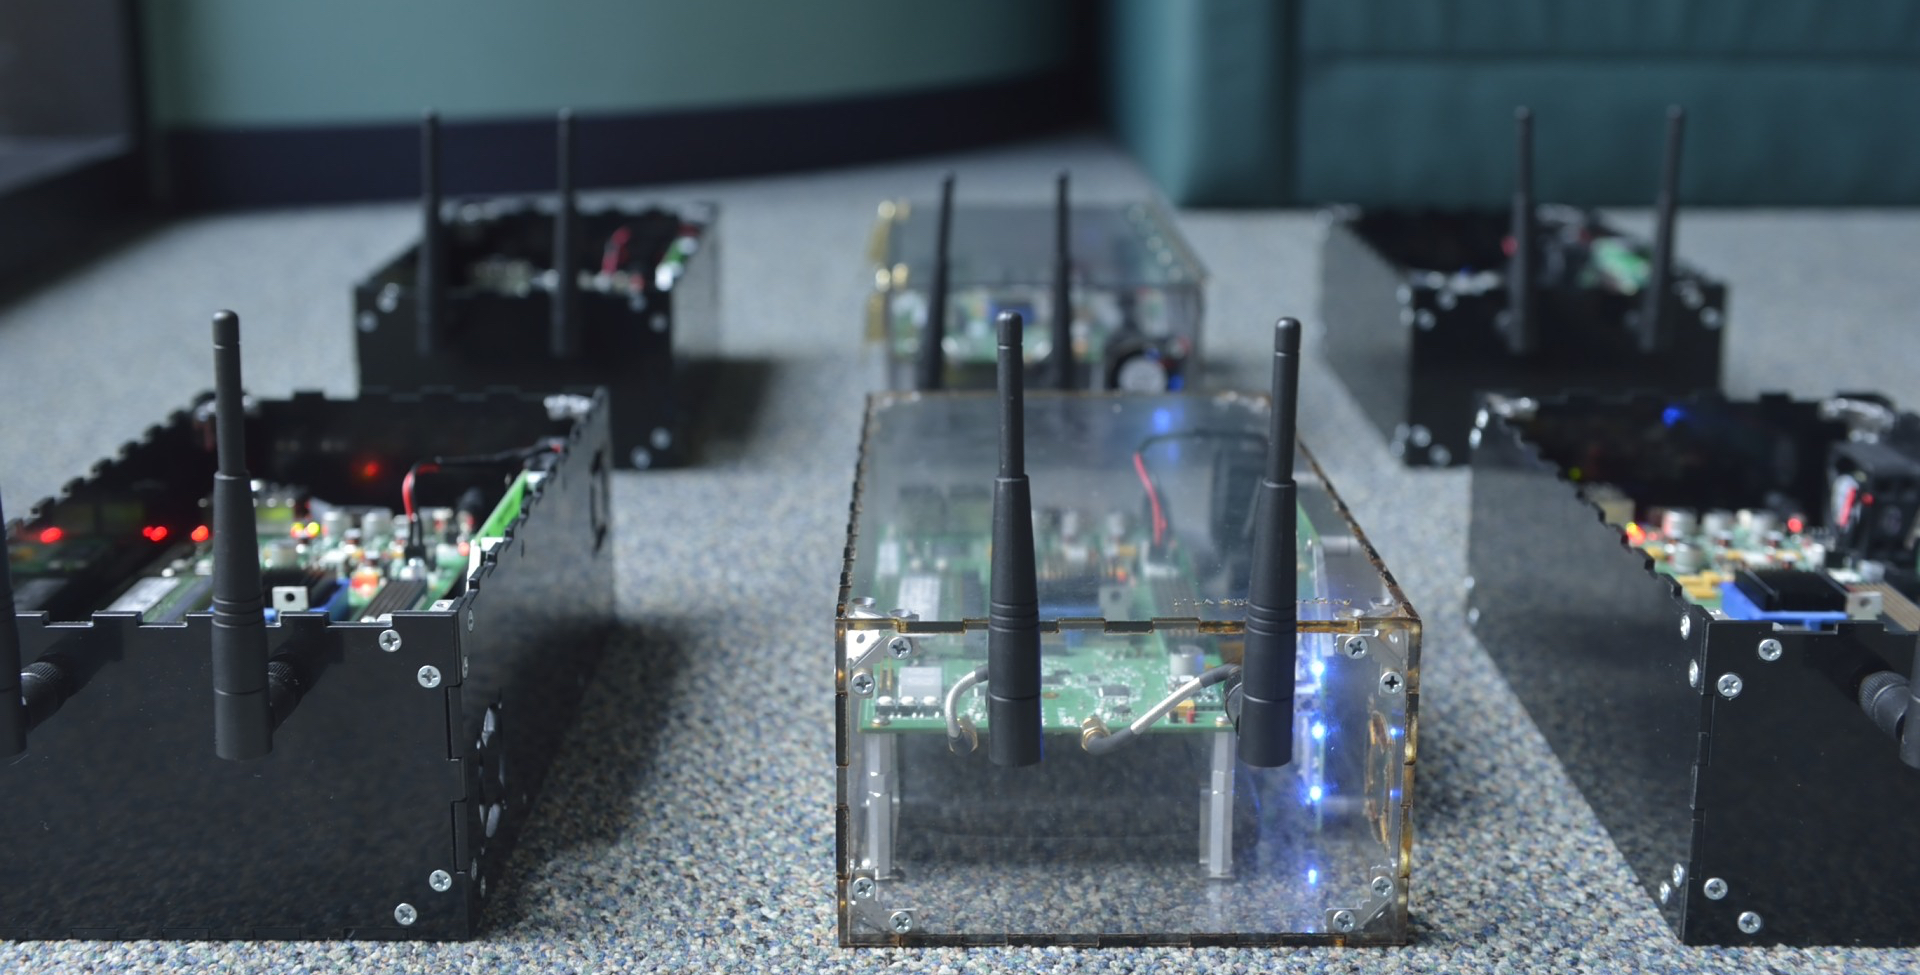
\includegraphics[width=0.95\textwidth]{ArgosMobile}
  \vspace{-2mm}
\caption{\emph{Battery-powered ArgosMobile based WARPv3.}}
\label{fig:argosmobile}
\end{minipage}
\hspace{+3mm}
\begin{minipage}[t][6cm]{0.463\textwidth}
    \centering
 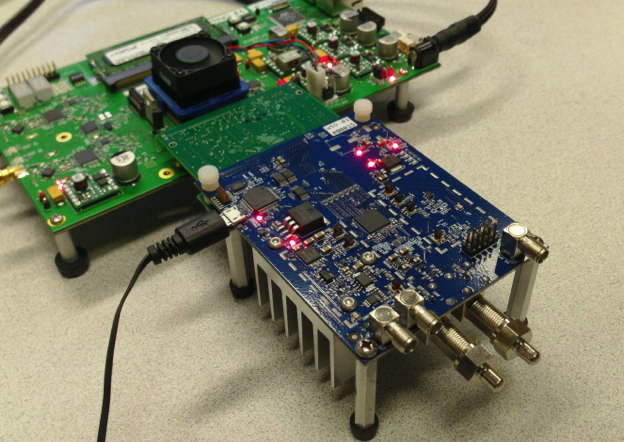
\includegraphics[width=0.95\textwidth]{WSD}
		\vspace{-2mm}
    \caption{\it{Volo wireless Whitespace daughtercard (WSD) adds UHF support to ArgosNet.}}
    \label{fig:WSD}
\end{minipage}
\vspace{-1mm}
\end{figure*}

\pagebreak
%\input{related}
% !TEX root = ../main.tex
%\pagebreak
\section{Education and Outreach Plan\label{sec:education}}
Our educational plan consists of three components, each tightly integrated with our research: (1) teaching embedded systems, wireless communication, and parallel and distributed systems, (2) engaging undergraduates and youth in research, and (3) encouraging female students in engineering.

The proposed project will contribute new curriculum content to the PIs' teaching in mobile computing, wireless communication, and parallel and distributed systems.  PI Zhang teaches senior elective courses ECE423 (Computer and Communication Networks) and ECE451 (Parallel and Distributed Computing) at Rutgers University. The proposed research will provide new lecture and laboratory modules for concepts in MIMO, radio tomography, vital sign sensing, and parallel applications. In particular, we plan to use diaster management as an application to drive communication protocol design and parallel computing in the two courses.  PI Zhong teaches a senior elective course ELEC/COMP424 Mobile \& Embedded System Design and Applications. The proposed research will provide new lecture and laboratory modules for concepts in distributed systems, hardware heterogeneity, and parallel programming. In particular, we plan to employ a face recognition application to teach about using specialized cores and synchronizing distributed states.


The proposed project will provide research opportunities to undergraduate students. PI Zhang has served as the faculty advisor for the Eta Kappa
Nu honor society for over 5 years. She has already worked with four undergraduate students from the honors program on related research projects, with publications coming out of several of these efforts (e.g.~\cite{jsspp03,sensorfusion05,xu:wise04,xu:mobihoc05}). PI Zhong has funded fifteen undergraduate students as research assistants in the past five years. Notably, he has four publications co-authored by undergraduates~\cite{rahmati2007mobilehci,liu2009percom,dong2009dac,dong2009islped} including two Best Paper awards~\cite{rahmati2007mobilehci,liu2009percom}. In this project, both teams plan to continue to work with undergraduate students. For each undergraduate assistant, we will define and tailor a project based on their interests, strengths, and career goals. Graduate students from both groups will work closely with undergraduates as collaborators and mentors. Moreover, we shall explore multiple funding opportunities for undergraduate research. Our track records include funding from the Brown Fund for Undergraduate Research, industry, and NSF REU supplements.

The proposed project will also provide a research platform to promote the awareness and interest in science and engineering among high-school students.  PI  Zhang has been engaged in an outreach to local high school students (Highland Park and Franklin High Schools in NJ). In this project, the Rutgers team will accept students from the Liberty Science Center's Partners in Science program and the WINLAB summer research program. PI Zhong will leverage his partnership with Harmony Science Academy, a local public school, to involve two students per semester in our research and mentor them for their Science Fair projects. PI Zhong has mentored five Harmony students in the past three years. One of them recently won the Second Place Award in Computer Science in the Texas Junior Academy of Science for her project under PI Zhong's guidance.


Ensuring that Science, Technology, Engineering and Mathematics (STEM) reaches as broad of a base as possible is an important activity that the investigators intend to focus on. PI Zhang has been actively involved in The Society of Women Engineers at Rutgers
University, where a series of workshops and luncheon meetings are
organized each semester, to give talks that emphasize the important
leadership roles open to women in EE/CS. She has supervised three female Ph.D. students, more than ten female master students and two female undergraduate students (both went to Cornell for graduate studies). One of her former Ph.D. students is now a tenured Associate Professor at University of South Carolina.
At CPS Week 2015, she served as one of the three panelists and discussed how to increase research impact for female researchers, which was very well received among female Ph.D. students and junior female faculty members. PI Zhong has also advised *** additional female PhD students. Moving forward, the PIs will continue their effort to encourage female students to engage in STEM.

\section{Broader Impact\label{sec:broader}}

The proposed project targets the following broader impact. We will leverage our collaborations with industry leaders in cyber-physical systems, including At\&T and Semens, to ensure a timely transfer of technologies and a broad impact on the commercial development of cyber physical systems. Our collaborations have already led to award-winning publications~\cite{liu2009percom,likamwa2011phonesense}, multiple patents, and likely product adoption.

We will publish research results and findings in academic conferences and journals and continue our tradition of demonstrating research results with prototypes at these conferences.
We plan to make our research hardware, software, and data open-source, as we have a strong record of doing this in the past. For example, PI Zhong have made the tools and data collected from~\cite{rahmati2007mobisys,liu2009percom,amirisani2010mobicom,shepard2010hotmetrics,wang2012www} open-source; PI Zhang has made the tools and data collected from~\cite{***} open-source.  More than 200 unique users have downloaded and used our data in their research according to CRAWDAD~\cite{crawdad}. Recently PI Zhong released the LiveLab data set, an extensive set of iPhone usage data from 34 users over six to 12 months~\cite{recgdownload}.

% !TEX root = ../main.tex
\section{Results from Prior NSF Supports\label{sec:prior}}

Both PIs Zhang and Zhong have received multiple NSF grants in the past five years. The most related to the proposed projects, one for each PI, are: 



In a NeTS Small project, \emph{LAWN: Scaling Up Cellular Data Networks
  using a Large Number of Antennas}, CNS-1218700 (2012-15). {\bf Intellectual Merit:}~~PI Zhong
investigate
network architecture issues in applying massive MU-MIMO to cellular
networks. This project produced the Argos 64-antenna MU-MIMO base station~\cite{shepard2012mobicom} and provided the early
results that motivate some of the proposed research activities~\cite{shepard2013cellnet}. {\bf Broader Impact:} Argos was the largest many-antenna MU-MIMO base station prototype publicly known at its publication~\cite{shepard2012mobicom}. It influenced Samsung's development of its own 32-antenna MU-MIMO base station prototype~\cite{samsung2013fdmimo} and recent 3GPP's approval of a proposal to study massive MIMO for LTE~\cite{fdmimo}. %s 

% Collaboration Plan
\clearpage
\pagenumbering{arabic}
\def\thepage{C-\arabic{page}}
% !TEX root = ../main.tex
\begin{center}
{\large {\bf Collaboration Plan}} \\
\end{center}
The proposed project team consists of two PIs (Yanyong Zhang and Lin Zhong), one senior personnel (XYZ), one postdoctoral researcher, and three graduate students. 

\subsection*{Team Expertise}
The two PIs and the senior personnel bring complementary expertise for the proposed research.

{\bf PI Yanyong Zhong}  


{\bf PI Lin Zhong} is a leading expert in mobile computing, including energy optimization and computer vision applications. His work has won best paper awards from ACM MobileHCI 2007~\cite{rahmati2007mobilehci}, IEEE PerCom 2009~\cite{liu2009percom}, ACM MobiSys 2011~\cite{dong2011mobisysa}, ACM MobiSys 2013~\cite{likamwa2013mobisysa}, ACM ASPLOS 2014~\cite{lin2014asplos}, and ACM MobiSys 2014~\cite{amirisani2014mobisys}.  In recent years, he has investigated operating system support for programming heterogeneous mobile SoC~\cite{lin2012asplos,lin2012hotpower,lin2014asplos}. This endeavor has not only led to early results for the proposed research but also led him and his team to realize the importance of programming system support for solving the problem. 

{\bf Senior Personnel XYZ} is the leading research scientist in 

{\bf Postdoctoral Researcher} support is included in the project budget. For this position, we will target at recruiting expertise in XYZ

\subsection*{Collaboration and Task Management}

PI Zhang will oversee the project and ensure its integration and success. 

\begin{figure}
    \centering
    \begin{minipage}[5cm]{0.44\textwidth}
    \centering
 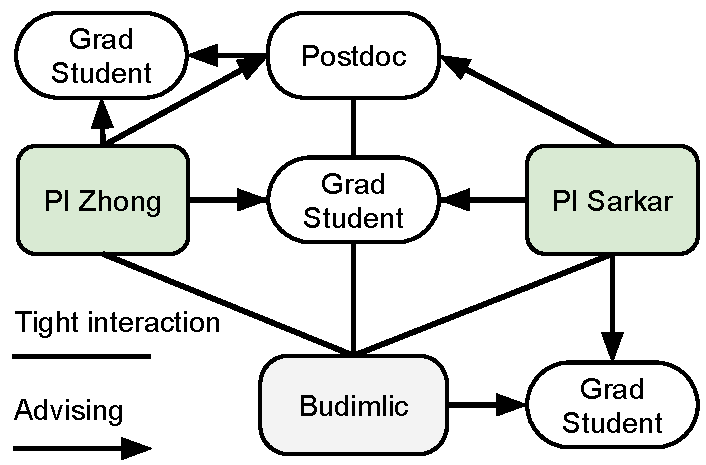
\includegraphics[height=0.17\textheight]{figs/collaboration}
%    \caption{\textit{Timeline for the proposed project}}
%    \label{fig:timeline}
    \end{minipage}
\hspace{+2mm}
    \begin{minipage}[5cm]{0.46\textwidth}    \centering
 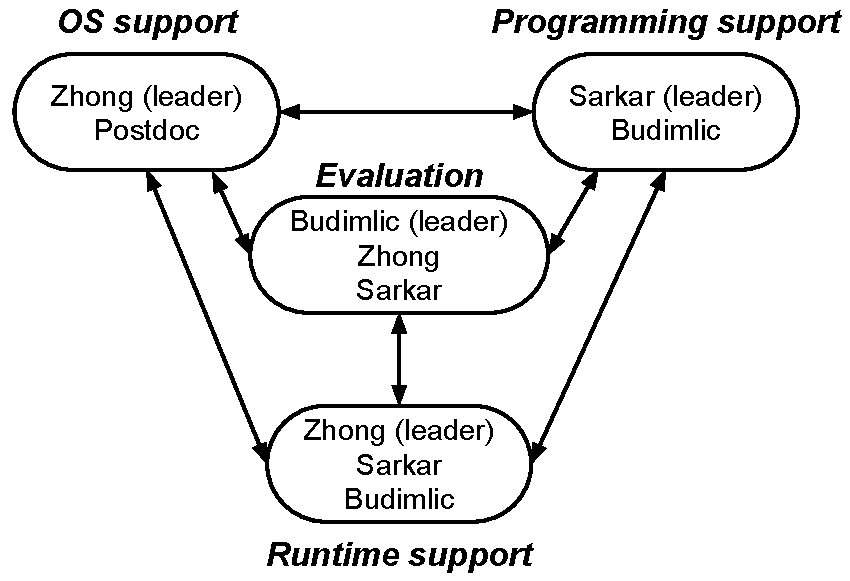
\includegraphics[height=0.18\textheight]{figs/taskmanagement}
    \end{minipage}
 \caption{\textit{(\emph{Left}) Graph of personnel and major interactions; and (\emph{Right}) Project task management with lead PI and participating PIs for each major research thrust.}}
    \label{fig:collaboration}
\end{figure}

While the two PIs have not had a joint NSF grant, they have already built a collaborative relationship due to their mutual interests in each other's research. 

\subsection*{Project Timeline\label{sec:management}}
The proposed project will be accomplished in four years. Figure~\ref{fig:timeline} presents the timeline for the major activities of the project. We emphasize the iterative nature of the three research thrusts and the evaluation plan because findings from one thrust are likely to change the course of another.  The education and outreach plan will be carried out through the four years.

%\begin{wrapfigure}{r}{0.75\textwidth}
%    \centering
% 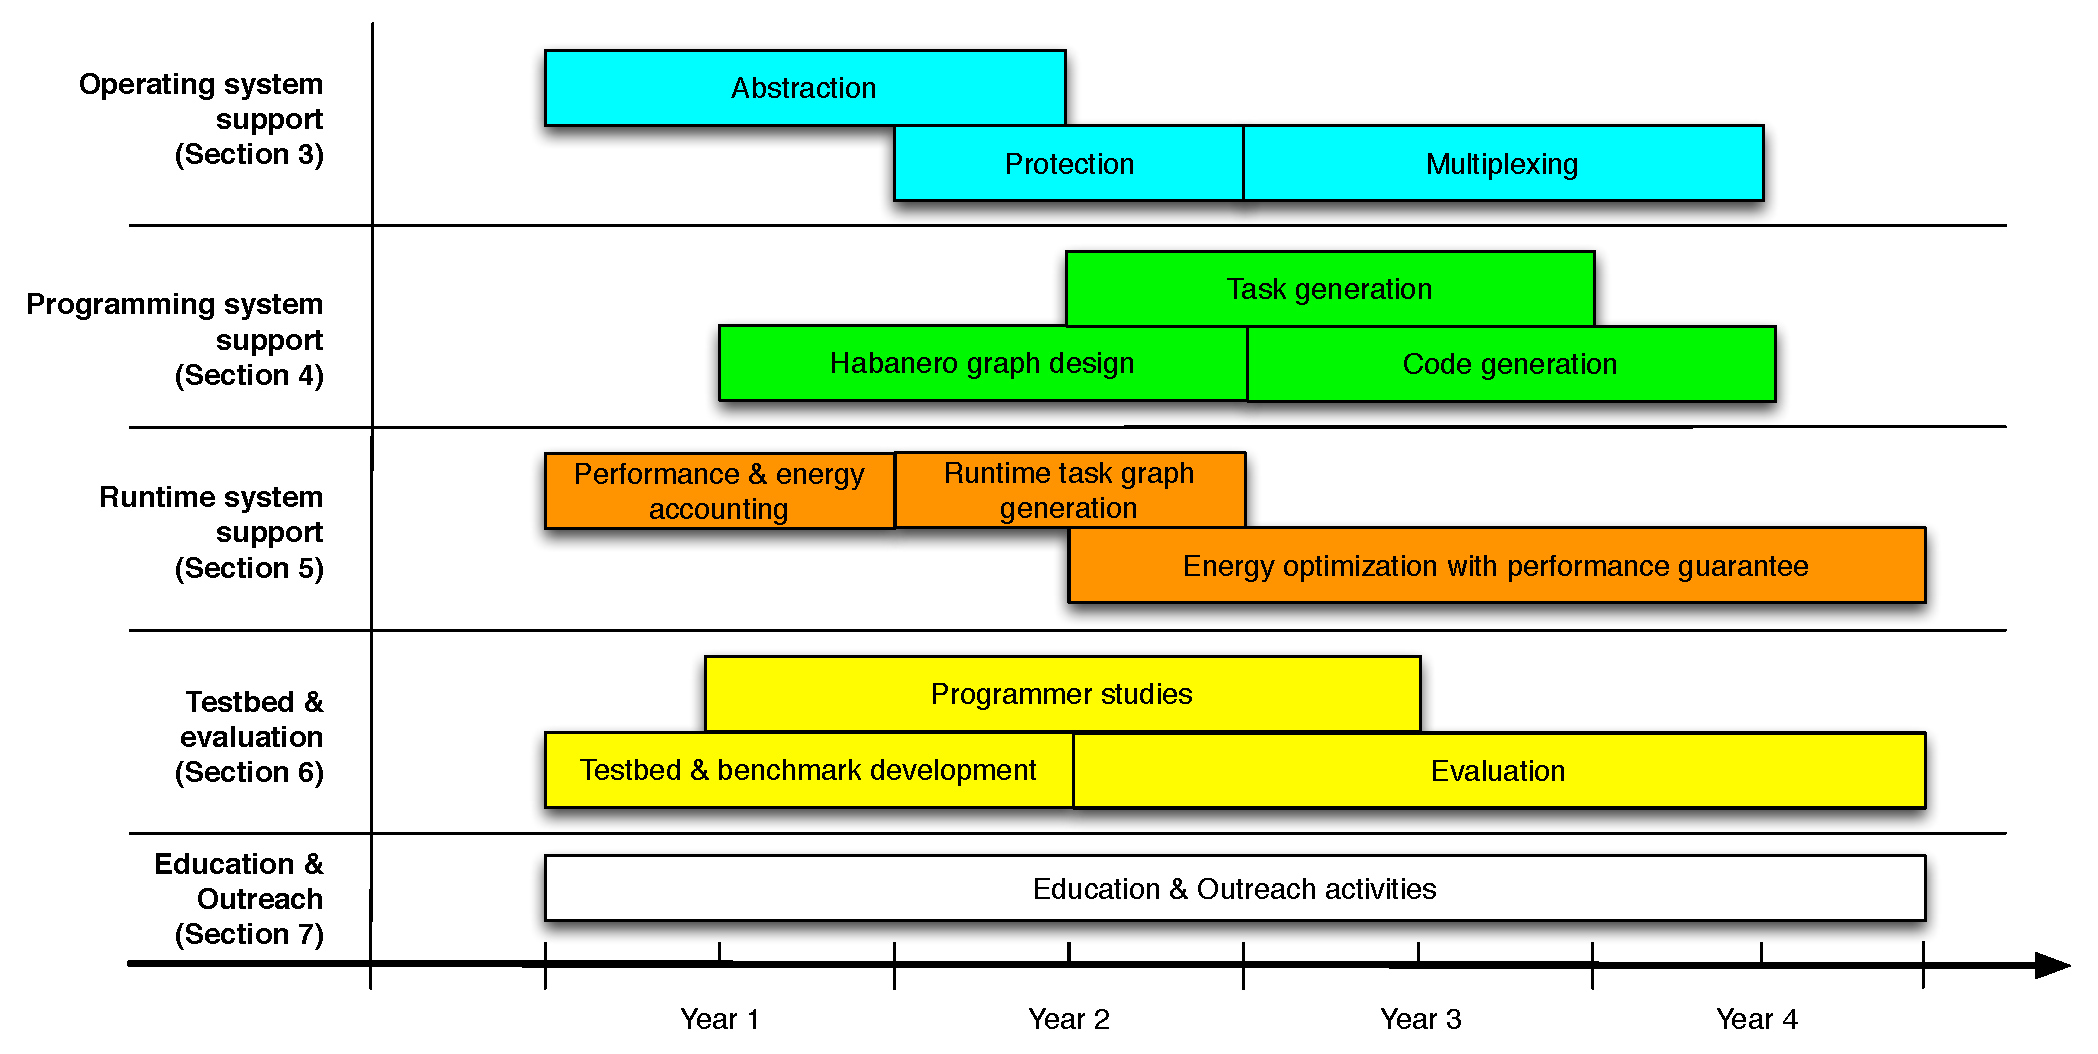
\includegraphics[width=0.75\textwidth]{figs/task-timeline}
%    \caption{\textit{Timeline for the proposed project}}
%    \label{fig:timeline}
%\end{wrapfigure}

\begin{figure}
    \centering
 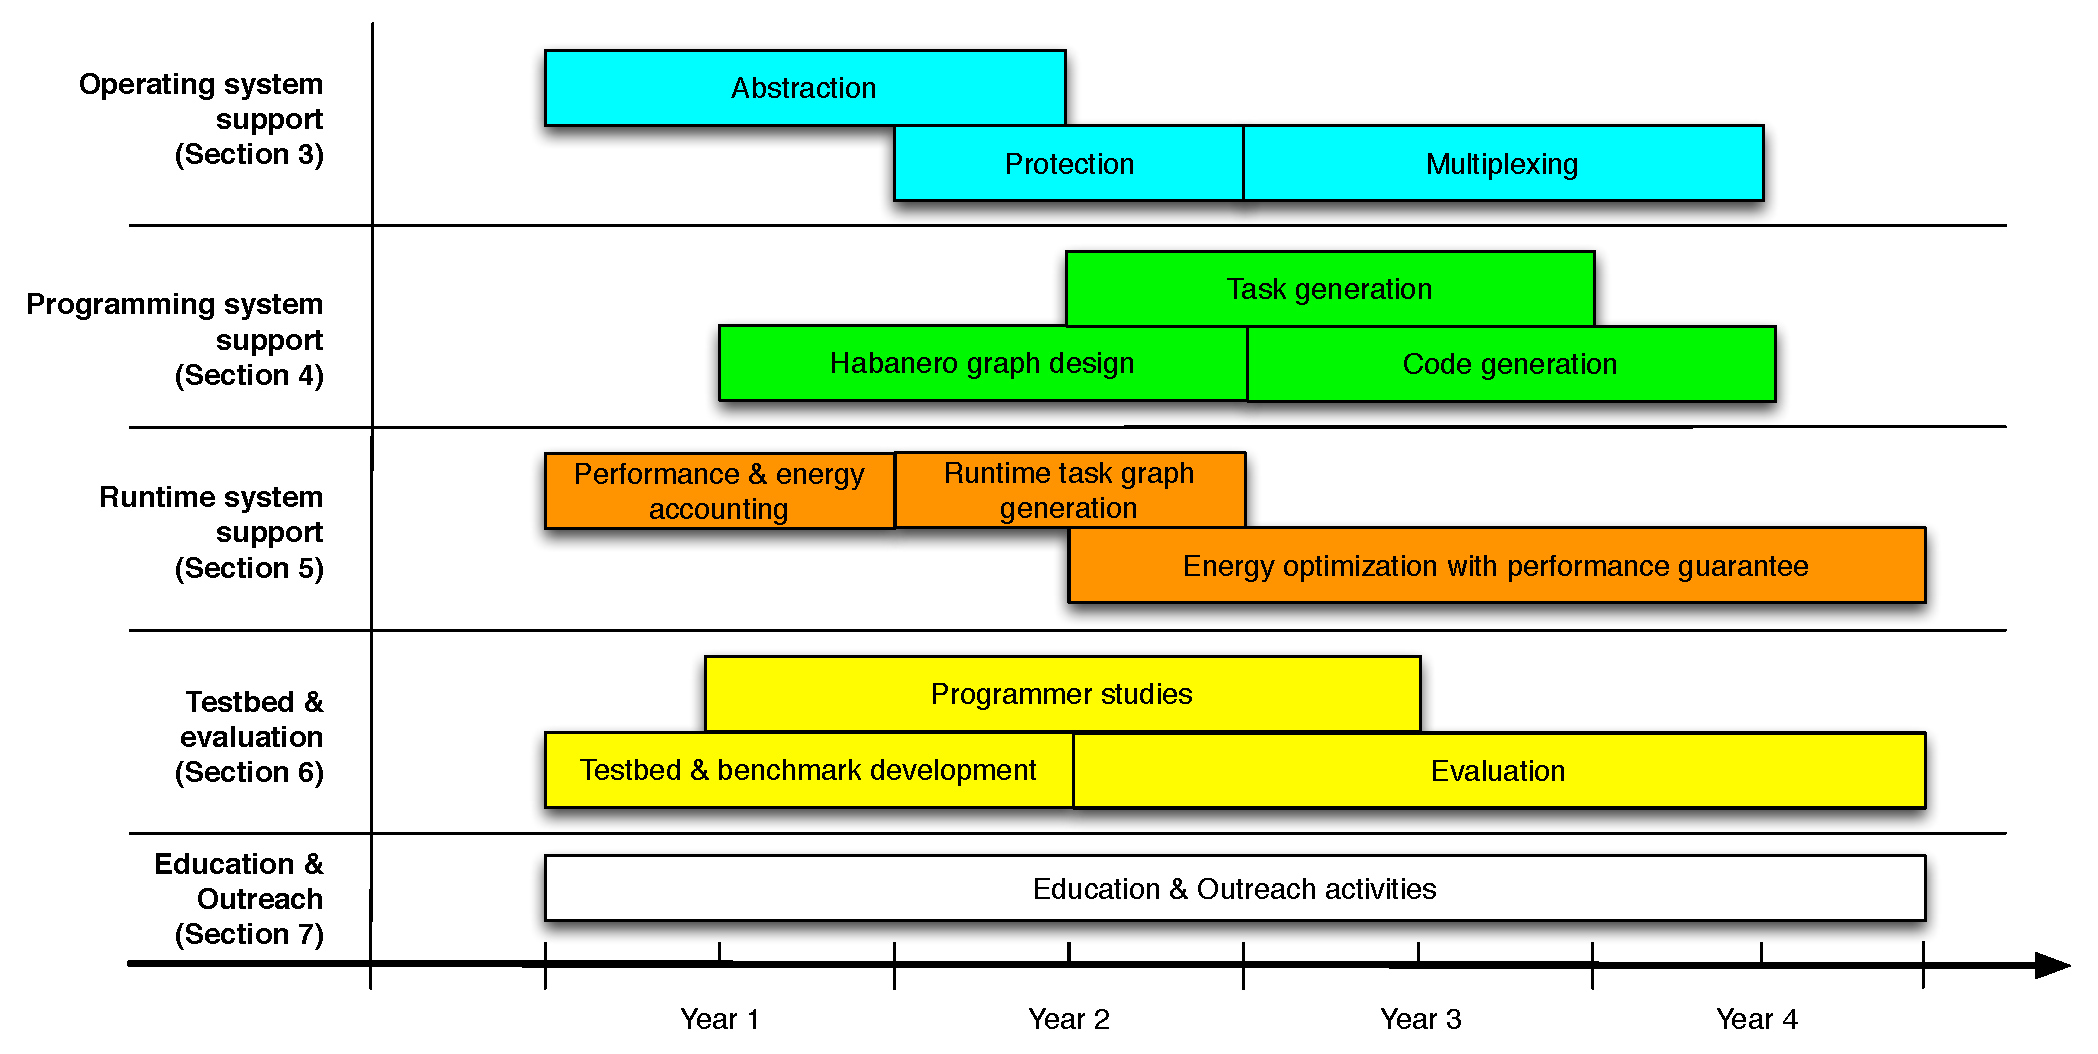
\includegraphics[width=0.75\textwidth]{figs/task-timeline}
    \caption{\textit{Timeline for the proposed project}}
    \label{fig:timeline}
\end{figure}

\subsection*{Coordination Mechanisms}
All members of the project team and their laboratories are located in the same building (Duncan Hall) on Rice campus, which greatly facilitates the project coordination. In addition, we will employ the following measures to ensure timely coordination of all research thrusts. (\textit{i}) First, we will use \emph{weekly team meeting} to foster face-to-face discussion and timely exchange of ideas. (\textit{ii}) Second, we will utilize  a \emph{Web-based internal collaboration system} called \emph{OWL-Space}~\cite{owlspace} to foster on-line discussion. Team members will also use this web system to provide weekly updates of their research and document milestones in their development.  (\textit{iii}) Third, we will use a \emph{Web-based public collaboration system (Wiki)} to host software and documentation releases to the public. It will also allow the public to provide feedbacks and foster a user community of the tools and software resulting from the proposed project. 


% Data Management Plan
\clearpage
\pagenumbering{arabic}
\def\thepage{D-\arabic{page}}
% !TEX root = ../main.tex
\begin{center}
{\bf \large Data Management Plan}
\end{center}

\subsection*{Types of Data}
The data obtained during the proposed project will consist of (\textit{i}) performance and power measurements from the testbeds running benchmark applications; and (\textit{ii}) programmer feedbacks in the form of survey and interview from the user study of mobile application developers. 

\subsection*{Data and Metadata Standards} 
While there are no existing standards for the type of data that we are dealing with, we shall nevertheless define and adopt a well-documented format for all the data and metadata that we create for simulation and testbed.

\subsection*{Policies for Access and Sharing}
Summaries of the data generated by the experiments will be available in the form of plots and statistics in peer-reviewed publications. Upon request, we will freely make available the associated data used for generating the results within a reasonable period of time. We will implement a web-based data dissemination policy in accord with the rules and regulations of Rice University. There will be no charge for accessing this data.  However, to limit the load on our server, we may place data rate or time of access restrictions. We retain the right to use the data before opening it up to wider use but once we publish a paper we will release its corresponding data. Further, we will extensively make use of the arXiv e-print archive (\url{http://www.arxiv.org}) to post our research results. 

We do not anticipate that there will be any significant intellectual property issues involved with the acquisition of the data. In the event that discoveries or inventions are made in direct connection with this data, access to the data will be granted upon request once appropriate invention disclosures and/or provisional patent filings have been made. 
The data acquired and preserved in the context of this proposal will be further governed by policies pertaining to intellectual property, record retention, and data management from Rice University.

The PIs have a track record for sharing research data and tools with the research community. For example, PI Zhong has made open-source the K2 operating system at http://www.k2os.org in addition to many others that are available from \url{http://www.recg.org}. For another example, we have released the tools and data collected from our papers that appeared in MobiSys 2007 and MobiCom 2010 at CRAWDAD (the Community Resource for Archiving Wireless Data At Dartmouth, URL: \url{http://crawdad.cs.dartmouth.edu/}). Over 300 users have downloaded and used our data in their research according to CRAWDAD. PI Sarkar also maintains an active website for the Habanero project at \url{http://habanero.rice.edu}, as well as a download site (\url{https://wiki.rice.edu/confluence/display/PARPROG/HJDownload}) for the  latest releases of Habanero Java and DrHJ.

\subsection*{Provisions for Human Subject Protection}
The proposed project will use mobile application developers as human subjects in order to evaluate the usability of the proposed programming languages and design flow. The data collected from these human subjects include interview, survey and basic demographic information. Such data along with the design of interview, survey, and the entire user study will be made open-access after proper anonymization to remove any identity revealing information, according to the requirement of the Rice University IRB approval. 

PI Zhong has a track record of sharing human subject data with the community after anonymization. For another example, his group has anonymized the iPhone usage data of 34 users over six months and made it open-access online (\url{http://livelab.recg.rice.edu}).  


\subsection*{Policies and Provisions for Re-use, Re-distribution}

There will be no permission restriction placed on the data, which will be freely accessible, usable for any purpose, and redistributable. To disseminate experimental code for operating system, compiler, runtime and other tools, the PIs will use the open-source public repository at the Habanero project at \url{http://habanero.rice.edu} and a publicly accessible Wiki. The experiment code, designs and implementations of testbed will be open-sourced under a derivate of FreeBSD-like non-viral license when possible. 


\subsection*{Plans for Archiving and Preservation of Access}
The data will be preserved for at least three years beyond the award period, as required by NSF guidelines. The long-term strategy for maintaining, curating and archiving the data is via regular backup of data sets into suitable long term storage media such as optical or magnetic media stored in a secure location separate from the database server. There are no transformations necessary to prepare the data for preservation/data sharing. As far as metadata goes documentation will be preserved alongside the data in order to make the data reusable.



% Postdoc Mentoring Plan
\clearpage
\pagenumbering{arabic}
\def\thepage{M-\arabic{page}}
% !TEX root = main.tex
\begin{center}
{\bf \large{Postdoctoral Researcher Mentoring Plan}} 
\end{center}


We have budgeted for one postdoctoral position. 
Our goal for the postdoctoral researcher mentoring program is to
provide exposure to a multi-disciplinary research program as well as
prepare the postdoctoral researcher for excelling in his/her chosen
career path.  To accomplish this goal, the mentoring plan will follow
the guidance of the National Postdoctoral
Association.\footnote{{http://www.nationalpostdoc.org/policy/institutional-policies/}} In
particular, we highlight following components:

\vspace{+2mm}

{\bf Multi-disciplinary training:}~~Our proposed research is in
  the intersection of systems, architecture, and security. The PIs are fully
  committed to training the postdoctoral researchers to be an expert in
  these areas. These efforts include regular, intense intellectual interactions
 between the researcher and the PIs in all areas, especially those
  where the researcher would like to particularly enhance his/her
  background and expertise. 
  Thus, the postdoctoral researcher will
  have ample opportunities to access both educational and research
  activities offered by the PIs.
  
\vspace{+2mm}

{\bf Support growth in professional network:}~~Having access to a
  large professional community is crucial to a researcher's career. To
  this end, we have budgeted adequate travel support for the
  postdoctoral researcher, so that he/she can attend important
  conferences in appropriate areas as well as visit other
  institutions to disseminate research results. The PIs will also
  encourage collaboration between the postdoctoral researcher and
  research communities  as
  well as the industry. The PIs will also designate certain research
  related administrative responsibilities, such as inviting and
  hosting well-known researchers, to increase the postdoctoral
  researcher's visibility and exposure to a larger professional
  network.
  
\vspace{+2mm}

{\bf Academic career preparation:}~~Preparing entry into the academic
  career path can be a challenging, painstaking, and sometimes
  confusing process. The PIs are committed to guiding the postdoctoral
  researchers in every phase and aspect of that process. The PIs
 have been on
  several faculty recruiting committees.  
  Our specific initiatives for enhancing the postdoctoral researcher's
  academic profile include integration into teaching (through guest
  lecturing, for instance), co-advising of Ph.D. students,
  participation in grant proposal and interview preparation.
  
  \vspace{+2mm}
{\bf Quality control and monitoring:}~~The PIs will assess the success
  of the mentoring plan by tracking the postdoctoral researcher's
  progress, according to an initially established plan and subsequent
  progress towards his/her chosen career path.
  
  
\vspace{+2mm}
{\bf Outreach and diversity activities:}~~We will make a
  significant effort to attract and recruit participation from
  traditionally underrepresented minorities in engineering, and
  particularly women. We will encourage the postdoctoral researcher 
  to participate in the outreach activities outlined in the project description
  and in particular be an informal mentor for students from underrepresented populations. 

% Facilities
\clearpage
\pagenumbering{arabic}
\def\thepage{F-\arabic{page}}
% !TEX root = ../main.tex
%\documentstyle{article}
%\begin{document}

\begin{center}
{\bf \large Facilities Overview}
\end{center}
\vspace{+2mm}
%\underline{\bf Overview}:
%\subsection*{Overview}


\section*{Rice Efficient Computing Group (Research Lab)}
PI Zhong directs the Rice Efficient Computing Lab. The lab is supported by funds and equipment from National Science Foundation, Rice University, Rice Computing Information Technology Institute, Microsoft Research, Motorola Labs, and Texas Instruments. The lab is currently equipped with the following hardware and software.\\

\noindent Hardware Resources:

\begin{itemize}
\vspace{-1.5mm}
\item  9 Dell PC workstations
\vspace{-1.5mm}
\item 2 Windows servers and 6 Linux servers
\vspace{-1.5mm}
\item 10 IBM/Lenovo laptops
\vspace{-1.5mm}
\item 10 Android smartphones and tablets of various makings

\vspace{-1.5mm}
\item 5 Texas Instruments PandaBoard and PandaBoard ES with OMAP4430 or OMAP4460

\vspace{-1.5mm}
\item 1 Texas Instruments Evaluation Board with OMAP5

\vspace{-1.5mm} 
\item 3 Google Glasses (with OMAP4430)
\vspace{-1.5mm} 
\item 2 Smart watches with Android Wear


\vspace{-1.5mm}
\item Data Acquisition System from Measurement Computing
\vspace{-1.5mm}
\item 2 Power Monitors from Mansoon Solutions
\vspace{-1.5mm}
\item Networked Data Acquisition System 2680A from Fluke Electronics, with proper software and peripherals
\vspace{-1.5mm}
\item One Argos Base Station Prototype including 15 WARPv2 boards
\end{itemize}

\noindent Software Resources:
\begin{itemize}
\vspace{-1.5mm}
\item  Microsoft Visual Studio 2008 (for Windows Mobile software development)
\vspace{-1.5mm}
\item Eagle PCB CAD tool
\vspace{-1.5mm}
\item IAR Embedded Workbench for TI MSP430
\vspace{-1.5mm}
\item Agilent ADS (a RF EDA tool of industrial strength)
\vspace{-1.5mm}
\item Cadence complete design tool chain with libraries
\vspace{-1.5mm}
\item QualNet 4.5 from Scalable Network Technologies for ultra high-fidelity network evaluation
\end{itemize}


\clearpage \pagenumbering{arabic}
\def\thepage{R-\arabic{page}}

\bibliographystyle{unsrt}

\bibliography{bib/abr,bib/zhong,bib/broader}


\end{document}


